\documentclass[conference]{IEEEtran}
 \IEEEoverridecommandlockouts

% Pacotes essenciais
\usepackage{cite}
\usepackage{amsmath,amssymb,amsfonts}
\usepackage{graphicx}
\usepackage{textcomp}
\usepackage{xcolor}

\def\BibTeX{{\rm B\kern-.05em{\sc i\kern-.025em b}\kern-.08em
    T\kern-.1667em\lower.7ex\hbox{E}\kern-.125emX}}

\begin{document}

\title{\textbf{Graph-Based Analyses of Brazilian Biomes Using Meteorological Data}}

\author{
    \IEEEauthorblockN{Rafael Adolfo Silva Ferreira}
    \IEEEauthorblockA{\textit{Department of Computer Science} \\
    \textit{Federal Center of Technological Education of Minas Gerais} \\
    Divinópolis, MG, Brazil \\
    Email: rafael.ferreira@aluno.cefetmg.br}
}

\maketitle

\begin{abstract}
Understanding the climatic distribution of Brazilian biomes is crucial for environmental monitoring and conservation strategies. This study proposes a graph-based approach to analyze the climatic similarities between different regions using meteorological data from INMET (Instituto Nacional de Meteorologia). By constructing a network where nodes represent meteorological stations and edges are weighted based on temperature and precipitation differences, we visualize biome connectivity and potential transitions. The results highlight significant overlaps between biomes such as the Amazon, Cerrado, and Atlantic Forest, suggesting the presence of ecotones. Additionally, a comparative analysis of graphs from 2012–2014 and 2020–2024 indicates possible climate-driven shifts, potentially influenced by deforestation and climate change. Despite data limitations, this methodology provides valuable insights into biome classification and environmental changes. Future research should refine climate weighting, incorporate additional variables like humidity and solar radiation, and integrate remote sensing for improved ecological modeling.
\end{abstract}

\begin{IEEEkeywords}
Brazilian biomes, graph theory, meteorological data, climate similarity, environmental monitoring, biome classification, climate change, ecological networks.
\end{IEEEkeywords}



\section{Introduction}

\

Understanding Brazilian biomes is essential for monitoring environmental changes and developing effective conservation policies. Brazil harbors a unique climatic and ecological diversity, distributed among the Amazon, Cerrado, Atlantic Forest, Caatinga, Pantanal, and Pampa biomes \cite{penereiro2018seasonal}. This diversity is influenced by climatic factors such as temperature, precipitation, humidity, and solar radiation, which determine vegetation dynamics and ecosystem behavior. However, studies that systematically integrate these factors remain limited, especially those employing methodologies capable of capturing the spatial and temporal interrelations of climatic variables.

Graph theory emerges as a promising approach to model and analyze the connectivity and interdependence of biomes based on meteorological data. Recent analyses have demonstrated that complex networks can be employed to identify climate variability patterns in Brazil, revealing how different regions relate in terms of fluctuations in temperature, humidity, and radiation \cite{oliveira2023networks}. The application of cross-correlation coefficients to meteorological time series enables the creation of graphs where connections represent climatic similarities between different regions, allowing for the detection of emerging patterns and seasonal trends.

The feasibility of this method is further reinforced by studies that have used bioclimatic indices to map vegetation and ecological conditions on a large scale. \cite{caudullo2014geospatial} proposed a set of bioclimatic indices for ecosystem delineation in Europe using only climatic variables, demonstrating that this approach could be adapted for Brazil. Similarly, studies on the Caatinga biome indicate that changes in vegetation can be detected solely through meteorological variables and remote sensing techniques \cite{ganem2020mapping,silva2022mapping}.

Thus, the application of network-based approaches using meteorological data can provide valuable insights into the dynamics of Brazilian biomes, identifying changes driven by climatic factors and enabling the development of adaptive strategies for conservation and sustainable management. Moreover, this approach can be expanded to predict future biome shifts in response to global climate change.
\section{Methodology}

\

In this study, its aim to map the Brazilian biomes by constructing graphs that represent the climatic similarities between different regions. To achieve this, it utilize meteorological data from the Banco de Dados Meteorológicos (BDMEP) provided by the Instituto Nacional de Meteorologia (INMET). This dataset offers comprehensive historical records from various meteorological stations across Brazil.

\subsection{Data Collection and Preparation}

\subsubsection{Station Catalog}

\

 The algorithm begins by loading the station catalog, which includes information such as station ID, name, state, latitude, and longitude. This allows us to map each station to its geographical location.
\subsubsection{Meteorological Data}

\

For each station, was gathered data on total precipitation and maximum and minimum temperatures. These variables are crucial for our analysis as they influence biome distribution.

\subsubsection{Data Aggregation}

\

The collected data are aggregated to compute the mean values for each station, ensuring that each station is represented by a single set of average climatic parameters.

\subsection{Normalization and Weighting}

\

To standardize the data and ensure comparability between stations, we normalize the temperature and precipitation values using z-scores. Following the methodology proposed by \cite{whittaker1975communities}, was assign weights to these variables to calculate a weighted climatic distance between stations. In this study, where  the assign a weight of 0.6 to precipitation and 0.4 to temperature, reflecting their respective influences on biome distribution.
\subsection{Graph Construction}

\subsubsection{Nodes}

\


Each meteorological station is represented as a node in the graph. It was used the \texttt{GeoPandas} library for geoespacial data manipulation, facilitating the integration of station data with their respective geographical locations \cite{geopandas2023}.

Attributes such as location (city and state), geographical coordinates (latitude and longitude), and the associated biome are assigned to each node. Location and coordinate information are extracted from the meteorological station catalog. To determine the corresponding biome for each station, are performed a spatial join between the station coordinates and the map of Brazilian biomes, obtained through the MapBiomas project \cite{mapbiomas2025}. This approach allows for a detailed analysis of the spatial distribution of stations within the country's various biomes.
\subsubsection{Edges}

\

Edges between nodes are established based on the climatic distance calculated between stations. The distance is computed using the formula:

\begin{equation}
  \text{Distance} = \sqrt{w_{\text{precip}} \times (\Delta P)^2 + w_{\text{temp}} \times (\Delta T)^2}
  \label{eq1:whittaker}
\end{equation}
where \( \Delta P \) and \( \Delta T \) represent the differences in normalized precipitation and temperature between two stations, respectively. The weight (\( w \)) values are as previously defined.
\subsubsection{Edge Weights}

\

The inverse of the calculated distance is used to define the edge weights, ensuring that stations with more similar climatic conditions are more strongly connected in the graph.

\subsection{Visualization with Gephi}

\

For data visualization in Gephi, an edge weight filter was applied, ranging from 0.85 to 0.99, to display only the edges that indicate high similarity, suggesting that the connected cities share a similar meteorological climate. The partitioning was performed based on predefined biomes, as described in the node section for coloration. The layout algorithm used was Fruchterman-Reingold \cite{fruchterman1991graph}, already on disposition in the software, a force-directed method that simulates forces acting on nodes to produce aesthetically pleasing graph layouts.

The Fruchterman-Reingold algorithm models nodes as steel rings and edges as springs between them. Attractive forces, analogous to spring forces, pull connected nodes together, while repulsive forces, similar to electrical forces, push all nodes apart. The algorithm aims to minimize the system's energy by adjusting node positions until an equilibrium state is reached, resulting in a visually appealing layout. In this approach, the sum of the force vectors determines the direction in which a node should move. The step width, a constant, dictates how far a node moves in a single iteration. To ensure convergence, a "global temperature" is introduced to control the step width and the algorithm's termination. Initially, nodes move rapidly due to a higher temperature, but as the temperature decreases over iterations, movements become more subtle, allowing the system to settle into an equilibrium state. This cooling process ensures that the nodes eventually stabilize, resulting in an optimized graph layout \cite{fruchterman1991graph}.

\section{Results}

\

The resulting graphs were generated using data from 2000 to 2024. However, due to missing stations in the INMET catalog and sparse data before 2012, only the graphs for the periods 2012–2014 and 2020–2024 are presented


\begin{figure}[ht]
  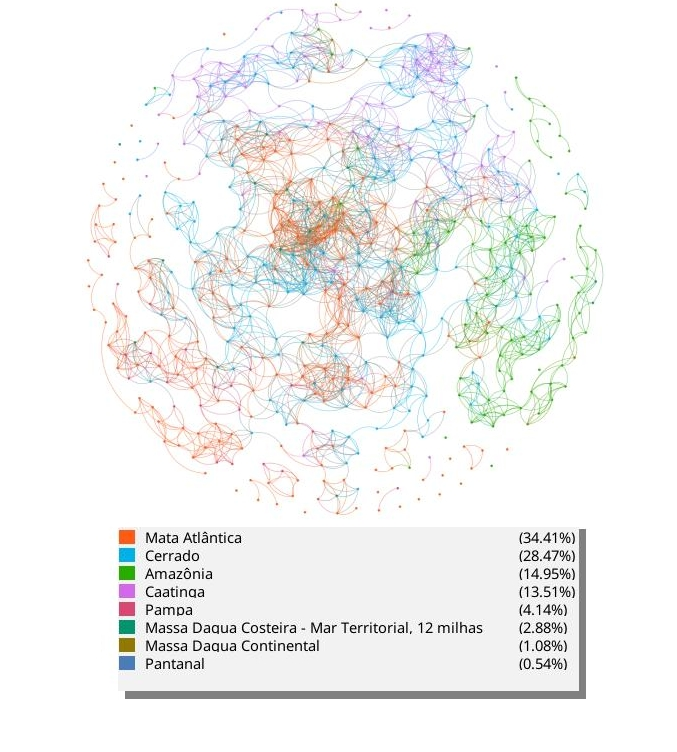
\includegraphics[width=0.53\textwidth]{imgs/20202024F.jpg}
  \caption{Graph resultant of 2020-2024.}
  \label{fig:example}
\end{figure}

\clearpage

\begin{figure}[ht]
  \centering
  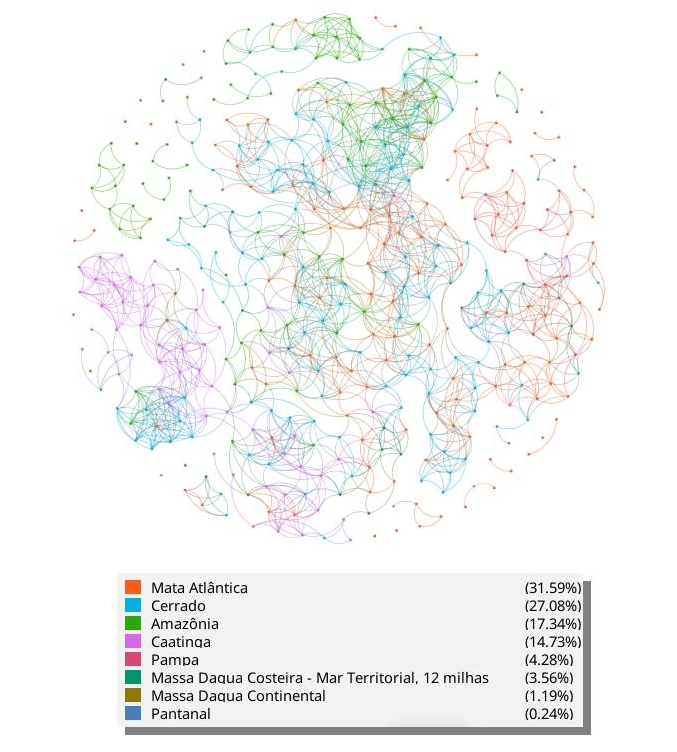
\includegraphics[width=0.53\textwidth]{imgs/20122014F.jpg}
  \caption{Graph resultant of 2012-2014.}
  \label{fig:g2}
\end{figure}

\


\section{Discussion}

The results obtained from the constructed graphs provide valuable insights into the climatic distribution of Brazilian biomes. However, some aspects require further investigation, particularly the high degree of overlap between biomes such as the Atlantic Forest, Cerrado, and Amazon. This entanglement suggests that certain meteorological stations share similar climate conditions despite belonging to different biomes. This phenomenon may be attributed to transitional zones or ecotones, which are regions where biomes gradually merge rather than having abrupt boundaries \cite{olson2001terrestrial}.

One possible explanation for the differences observed between the 2012-2014 and 2020-2024 graphs is the impact of climate change and deforestation. Studies indicate that Brazil has experienced significant variations in precipitation and temperature patterns over the last decades, influenced by anthropogenic activities and global climate shifts \cite{marengo2020extreme}. Deforestation in the Amazon, for instance, has been linked to reduced rainfall and increased temperatures, which could alter the connectivity of meteorological stations within the network \cite{nobre2016land}.

Additionally, the quality and availability of meteorological data could play a role in these discrepancies. The INMET dataset, while comprehensive, may suffer from station discontinuities, equipment calibration differences, or missing data, particularly in earlier periods. This may result in variations in graph density and connectivity over time \cite{sapucci2019quality}.

Another important consideration is the weight assignment in the climatic distance formula. The choice of 0.6 for precipitation and 0.4 for temperature, while justified based on Whittaker’s biome classification, may not fully capture biome dynamics in Brazil. Adjusting these weights or incorporating additional climate variables such as solar radiation could enhance the model's accuracy \cite{whittaker1975communities}.

Despite these limitations, the approach successfully highlights climatic similarities between regions, reinforcing the idea that network-based methods can effectively model ecological distributions. Future studies should aim to refine the methodology by incorporating more climate parameters and validating the results with ecological field data. Furthermore, integrating remote sensing techniques and land-use data may help in better understanding the long-term shifts in Brazilian biomes \cite{deoliveira2021remote}.

\section{Conclusion}

The application of graph-based methods to analyze Brazilian biomes has proven effective in visualizing climatic relationships between different regions. The constructed networks not only confirm expected biome distributions but also reveal nuanced climatic gradients and transitions. However, the observed overlap between biomes such as the Atlantic Forest, Cerrado, and Amazon underscores the complexity of these ecosystems and highlights the presence of transitional zones.

The differences identified between the 2012-2014 and 2020-2024 graphs suggest that climate change and deforestation are playing a crucial role in altering the connectivity of meteorological stations. Changes in precipitation and temperature patterns, coupled with land-use modifications, may be influencing biome boundaries over time. 

To improve the accuracy of biome mapping, future research should focus on refining the weighting of climate variables and incorporating additional factors such as humidity and solar radiation. Moreover, integrating remote sensing data and ecological field studies could provide a more comprehensive understanding of the dynamic shifts occurring within Brazilian biomes. This study reinforces the importance of climate-based classification methods and highlights the need for continuous monitoring to assess the long-term impacts of environmental change on biome distribution.

\begin{thebibliography}{00}

  \bibitem{scheiter2024crowd} 
  S. Scheiter, S. Wolf, and T. Kattenborn, “Crowd-sourced trait data can be used to delimit global biomes,” *Biogeosciences*, vol. 21, no. 21, pp. 4909--4926, 2024, doi: 10.5194/bg-21-4909-2024.
  
  \bibitem{bonannella2023biomes} 
  C. Bonannella, T. Hengl, L. Parente, and S. de Bruin, “Biomes of the world under climate change scenarios: increasing aridity and higher temperatures lead to significant shifts in natural vegetation,” *PeerJ*, vol. 11, p. e15593, 2023, doi: 10.7717/peerj.15593.
  
  \bibitem{kottek2006world} 
  M. Kottek, J. Grieser, C. Beck, B. Rudolf, and F. Rubel, “World map of the Köppen-Geiger climate classification updated,” *Meteorologische Zeitschrift*, vol. 15, no. 3, pp. 259--263, 2006, doi: 10.1127/0941-2948/2006/0130.
  
  \bibitem{olson2001terrestrial} 
  D. M. Olson et al., “Terrestrial ecoregions of the world: a new map of life on Earth,” *BioScience*, vol. 51, no. 11, pp. 933--938, 2001, doi: 10.1641/0006-3568(2001)051[0933:TEOTWA]2.0.CO;2.
  
  \bibitem{southworth2023latitudes} 
  J. Southworth et al., “Latitudes and land use: Global biome shifts in vegetation persistence across three decades,” *Frontiers in Remote Sensing*, vol. 4, p. 1063188, 2023, doi: 10.3389/frsen.2023.1063188.
  
  \bibitem{oliveira2023networks} 
  F. M. Oliveira Filho, E. F. Guedes, and P. C. Rodrigues, “Networks analysis of Brazilian climate data based on the DCCA cross-correlation coefficient,” *PLoS ONE*, vol. 18, no. 9, p. e0290838, 2023, doi: 10.1371/journal.pone.0290838.
  
  \bibitem{penereiro2018seasonal} 
  J. C. Penereiro, A. Badinger, N. A. Maccheri, and M. C. Meschiatti, “Distributions of Seasonal Average Temperature and Precipitation Trends in Brazilian Biomes,” *Revista Brasileira de Meteorologia*, vol. 33, no. 1, pp. 97--113, 2018, doi: 10.1590/0102-7786331012.
  
  \bibitem{caudullo2014geospatial} 
  G. Caudullo, “Applying Geospatial Semantic Array Programming for a Reproducible Set of Bioclimatic Indices in Europe,” *IEEE Earthzine*, vol. 7, no. 2, 2014. [Online]. Available: http://www.earthzine.org/?p=877975.
  
  \bibitem{ganem2020mapping} 
  K. A. Ganem et al., “Mapping Caatinga Vegetation using Optical Earth Observation Data – Opportunities and Challenges,” *Revista Brasileira de Cartografia*, vol. 72, 2020, doi: 10.14393/rbcv72nespecial50anos-56543.
  
  \bibitem{silva2022mapping} 
  U. J. da Silva Júnior, R. C. da Fonseca, and J. A. da Silva Júnior, “Mapping of Caatinga Biome Vegetation through NDVI MODIS Time Series and Albedo, in Pajeú River Basin - PE, BR,” *Caminhos de Geografia*, vol. 23, no. 90, pp. 75–89, 2022, doi: 10.14393/RCG239060898.
  
  \bibitem{whittaker1975communities} 
  R. H. Whittaker, *Communities and Ecosystems*. Toronto: MacMillan Publishing, 1975.
  
  \bibitem{geopandas2023} 
  J. Van den Bossche et al., “GeoPandas: Python tools for geographic data,” 2023. [Online]. Available: https://geopandas.org/.
  
  \bibitem{mapbiomas2025} 
  “MapBiomas Brazil,” 2025. [Online]. Available: https://brasil.mapbiomas.org/en/.
  
  \bibitem{fruchterman1991graph} 
  T. M. J. Fruchterman and E. M. Reingold, “Graph Drawing by Force-directed Placement,” *Software: Practice and Experience*, vol. 21, no. 11, pp. 1129--1164, 1991, doi: 10.1002/spe.4380211102.
  
  \bibitem{bastian2009gephi} 
  M. Bastian, S. Heymann, and M. Jacomy, “Gephi: An Open Source Software for Exploring and Manipulating Networks,” in *International AAAI Conference on Weblogs and Social Media*, 2009. [Online]. Available: https://gephi.org.
  
  \bibitem{marengo2020extreme} 
  J. A. Marengo et al., “Extreme climatic and weather events in Brazil,” *Frontiers in Earth Science*, vol. 8, 2020, pp. 1--15.
  
  \bibitem{nobre2016land} 
  C. A. Nobre et al., “Land-use and climate change risks in the Amazon and the need of a novel sustainable development paradigm,” *Proceedings of the National Academy of Sciences*, vol. 113, no. 39, pp. 10759--10768, 2016.
  
  \bibitem{sapucci2019quality} 
  L. F. Sapucci et al., “Quality control of meteorological data from INMET,” *Brazilian Journal of Meteorology*, vol. 34, pp. 527--543, 2019.
  
  \bibitem{deoliveira2021remote} 
  G. de Oliveira et al., “Remote sensing for biome monitoring in Brazil,” *Remote Sensing*, vol. 13, 2021, pp. 1--19.
  
  \end{thebibliography}
  

\end{document}
